\documentclass[../FinalThesis.tex]{subfiles}
\begin{document}

%------------------------------------------------------------------------------
%	Appendix S1:
%------------------------------------------------------------------------------
\newpage
\section{Landscape Simulation: Different Autocorrelation Scenarios}
\begin{figure}[!ht]
  \begin{center}
  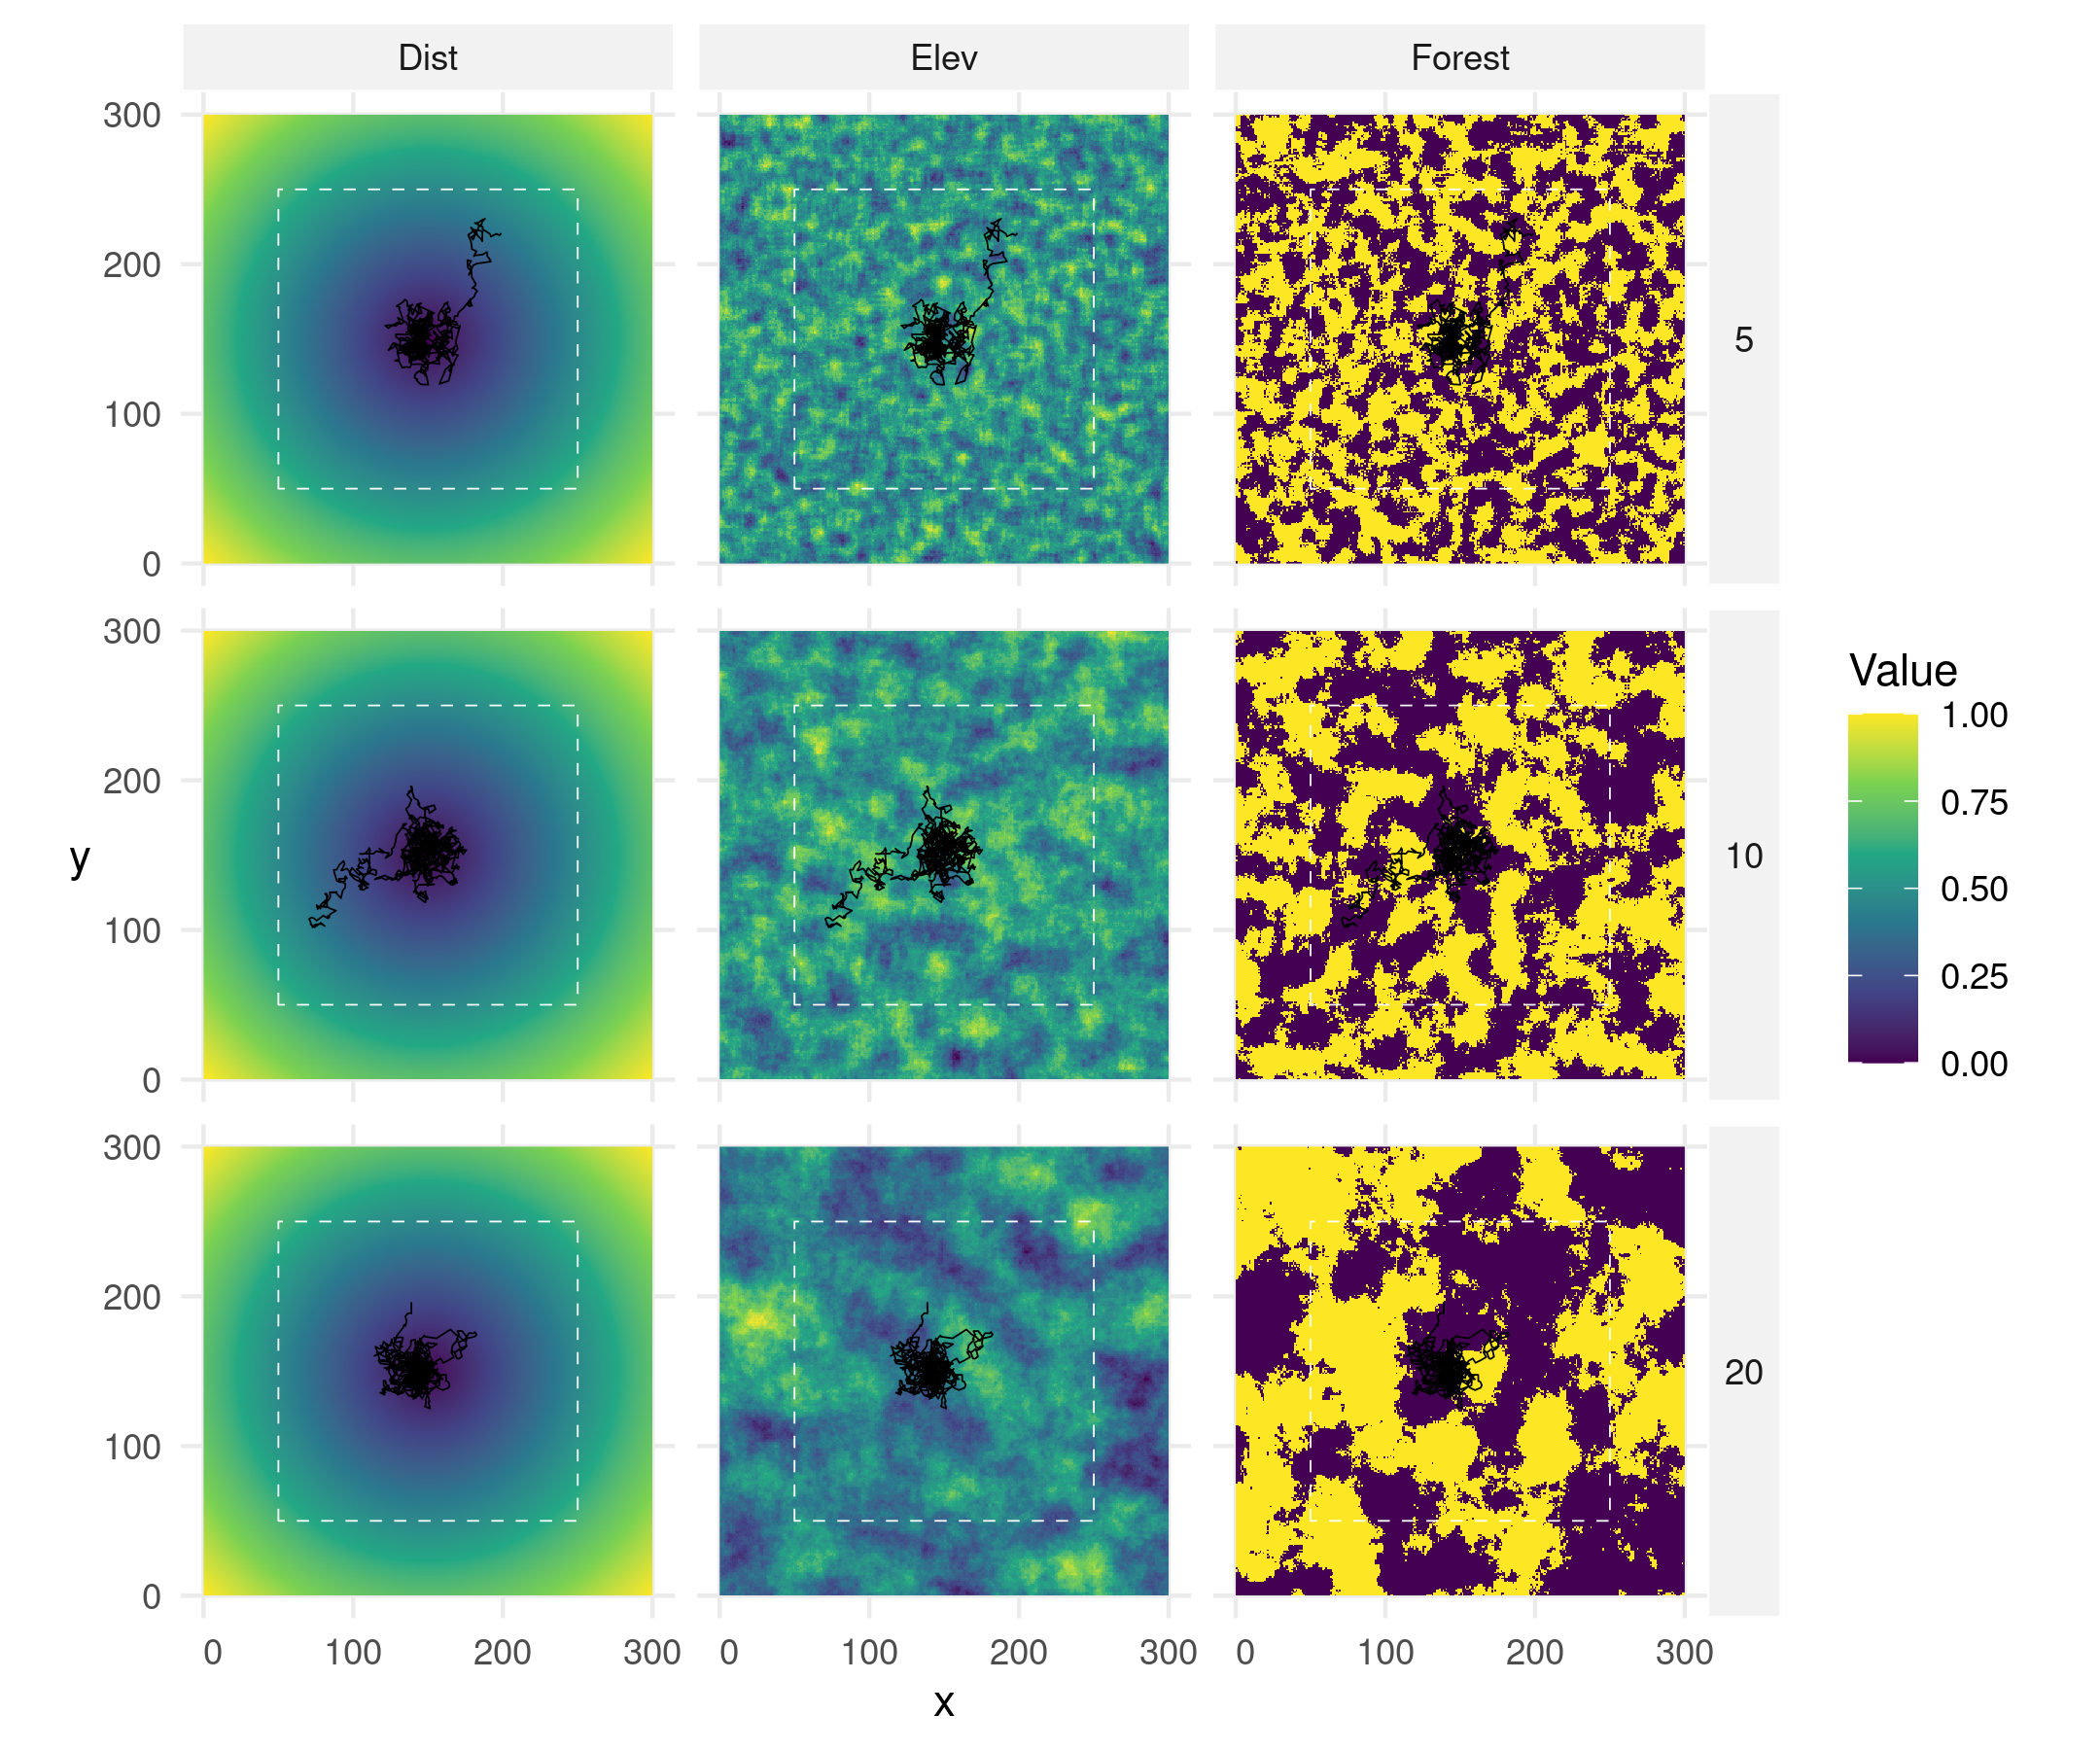
\includegraphics[width = \textwidth]{Figures/CovariatesAppendix.png}
  \caption{Simulated landscapes under different levels of autocorrelation (5,
  10, 20; from top to bottom). Autocorrelation only affected the layers
  \textsf{elev} and \textsf{forest}, which were both simulated using a Gaussian
  random field neutral landscape model \citep{Schlather.2015} using the
  \texttt{R}-package \texttt{NLMR} \citep{Sciaini.2018}. Simulations were
  repeated 100 times for each autocorrelation scenario, thus resulting in 300
  unique landscape configurations.}
  \label{SimulatedCovariates}
  \end{center}
\end{figure}

%------------------------------------------------------------------------------
%	Appendix S2:
%------------------------------------------------------------------------------
\newpage
\section{Dynamic Tentative Distribution Parameters}
\begin{figure}[!ht]
  \begin{center}
  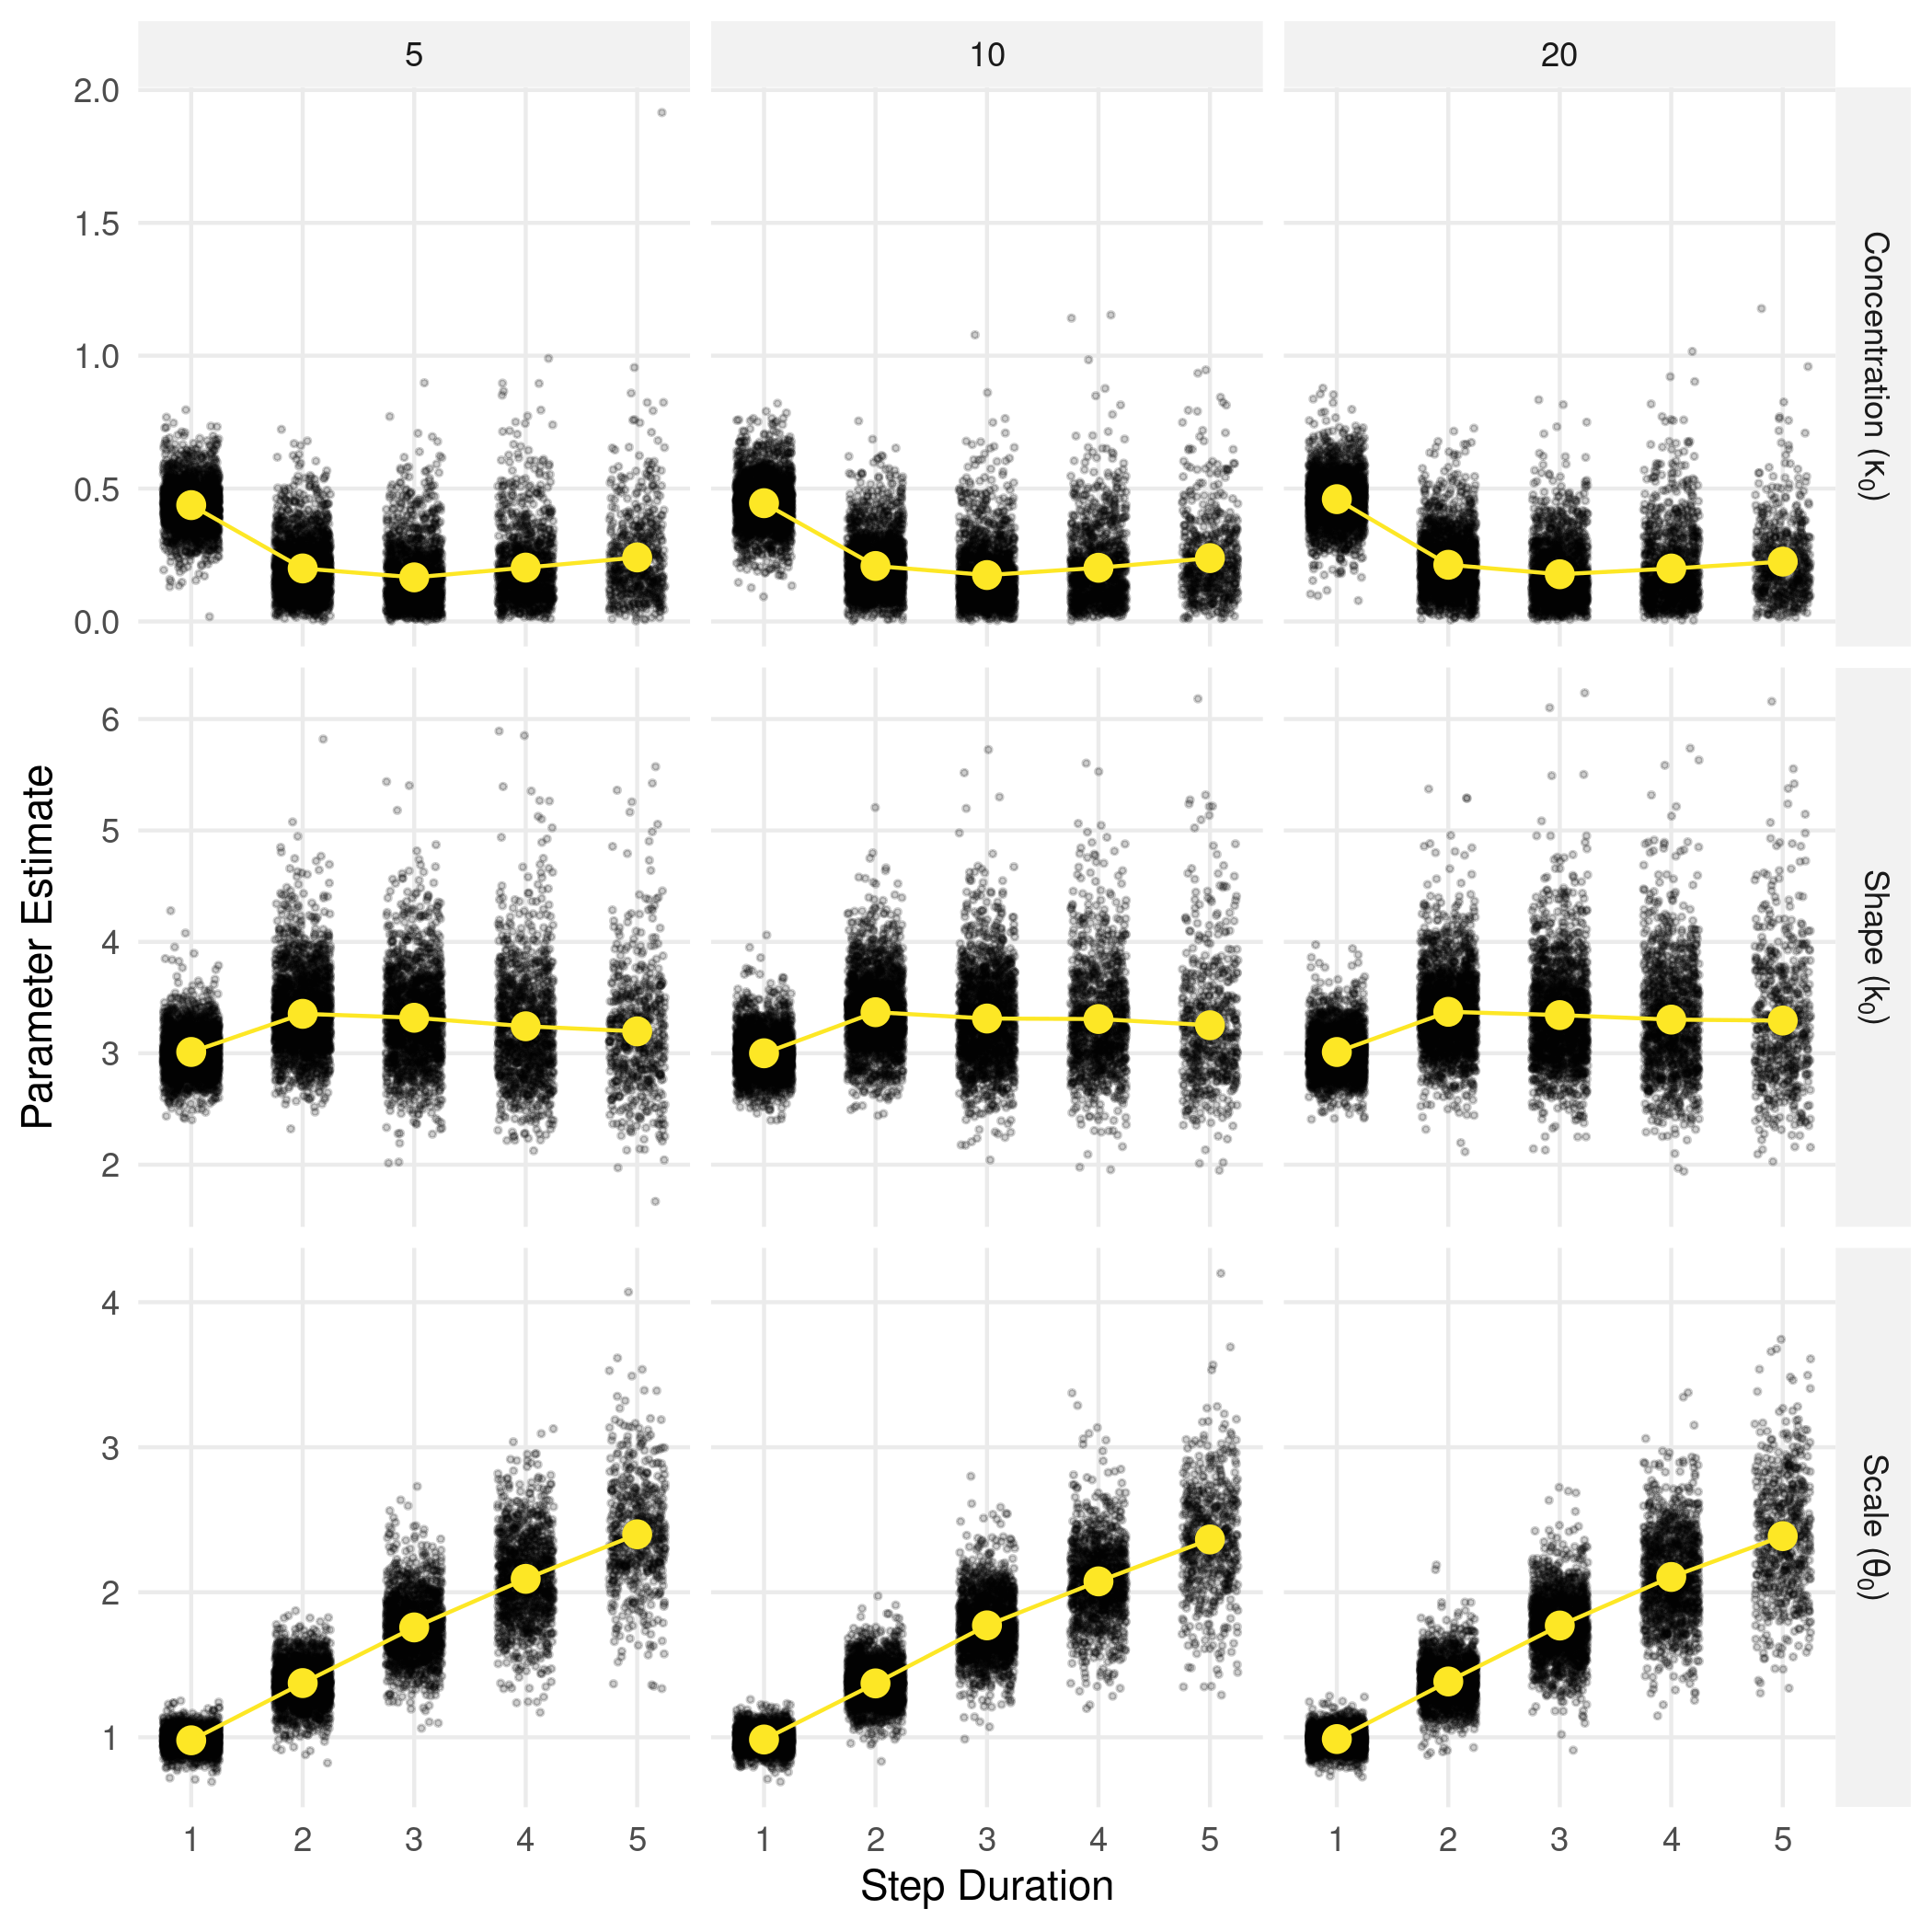
\includegraphics[width = 0.9\textwidth]{Figures/DistributionParameters.png}
  \caption{Tentative prameter estimates for the von Mises distribution (top row) and
  gamma distribution (bottom row) fitted to steps with different durations. The
  von Mises distribution requires one parameter, namely a concentration
  parameter ($\kappa$). The gamma distribution requires a shape parameter ($k$)
  and a scale parameter ($\theta$). The subscript $_0$ is used to indicate that
  these are tentative distribution parameters (sensu \citealp{Avgar.2016} and
  \citealp{Fieberg.2021}).}
  \label{DistributionParameters}
  \end{center}
\end{figure}

%------------------------------------------------------------------------------
%	Appendix S3:
%------------------------------------------------------------------------------
\newpage
\section{Distribution of Relative Turning Angles following Different Step Durations}
\begin{figure}[!ht]
  \begin{center}
  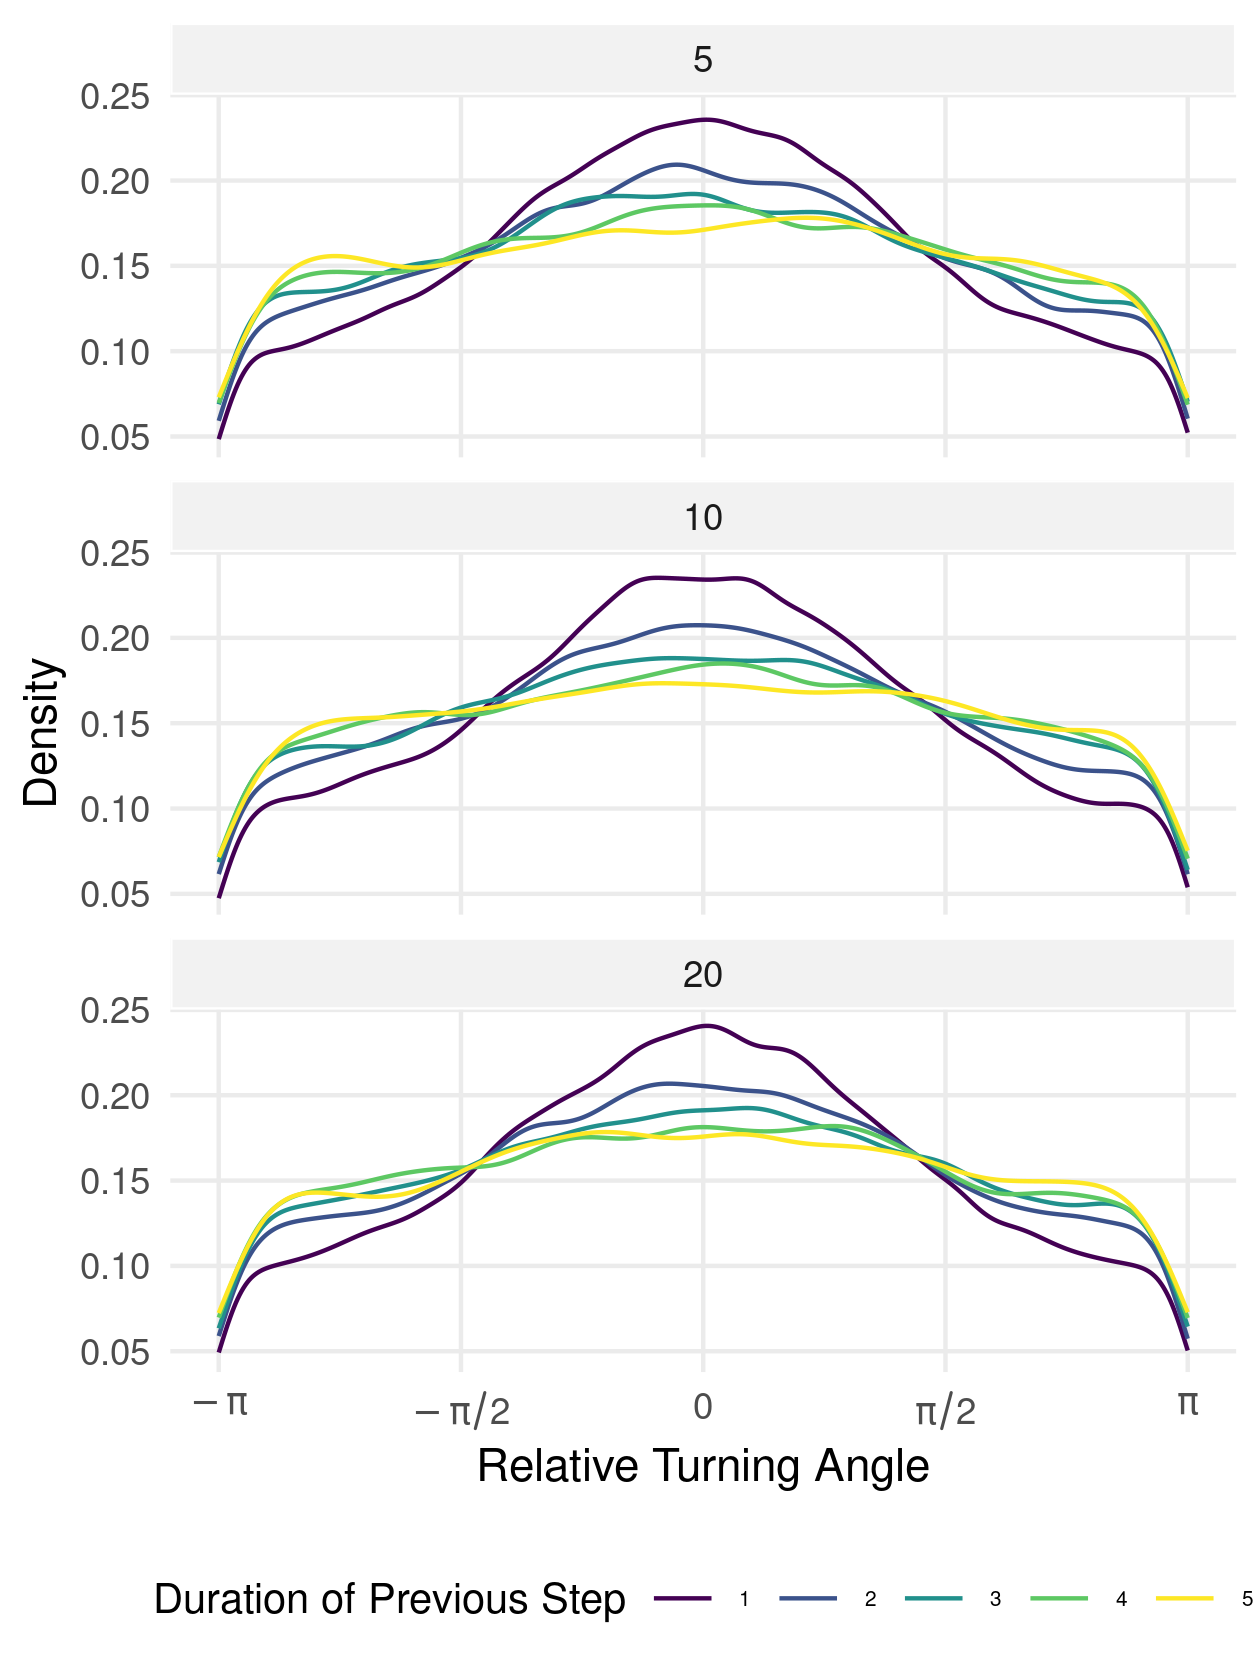
\includegraphics[width = 0.8\textwidth]{Figures/TurningAnglePreviousDuration.png}
  \caption{Density of relative turning angles associated with steps of $\Delta t
  = 1$ following steps with different durations for all three autocorrelation
  scenarios (5, 10, and 20). To generate this figure, we assumed a missingness
  of 0.5 and forgiveness of 5.}
  \label{PreviousDuration}
  \end{center}
\end{figure}

%------------------------------------------------------------------------------
%	Appendix S4:
%------------------------------------------------------------------------------
\newpage
\section{Model Estimates across all Scenarios}
\begin{figure}[!ht]
  \begin{center}
  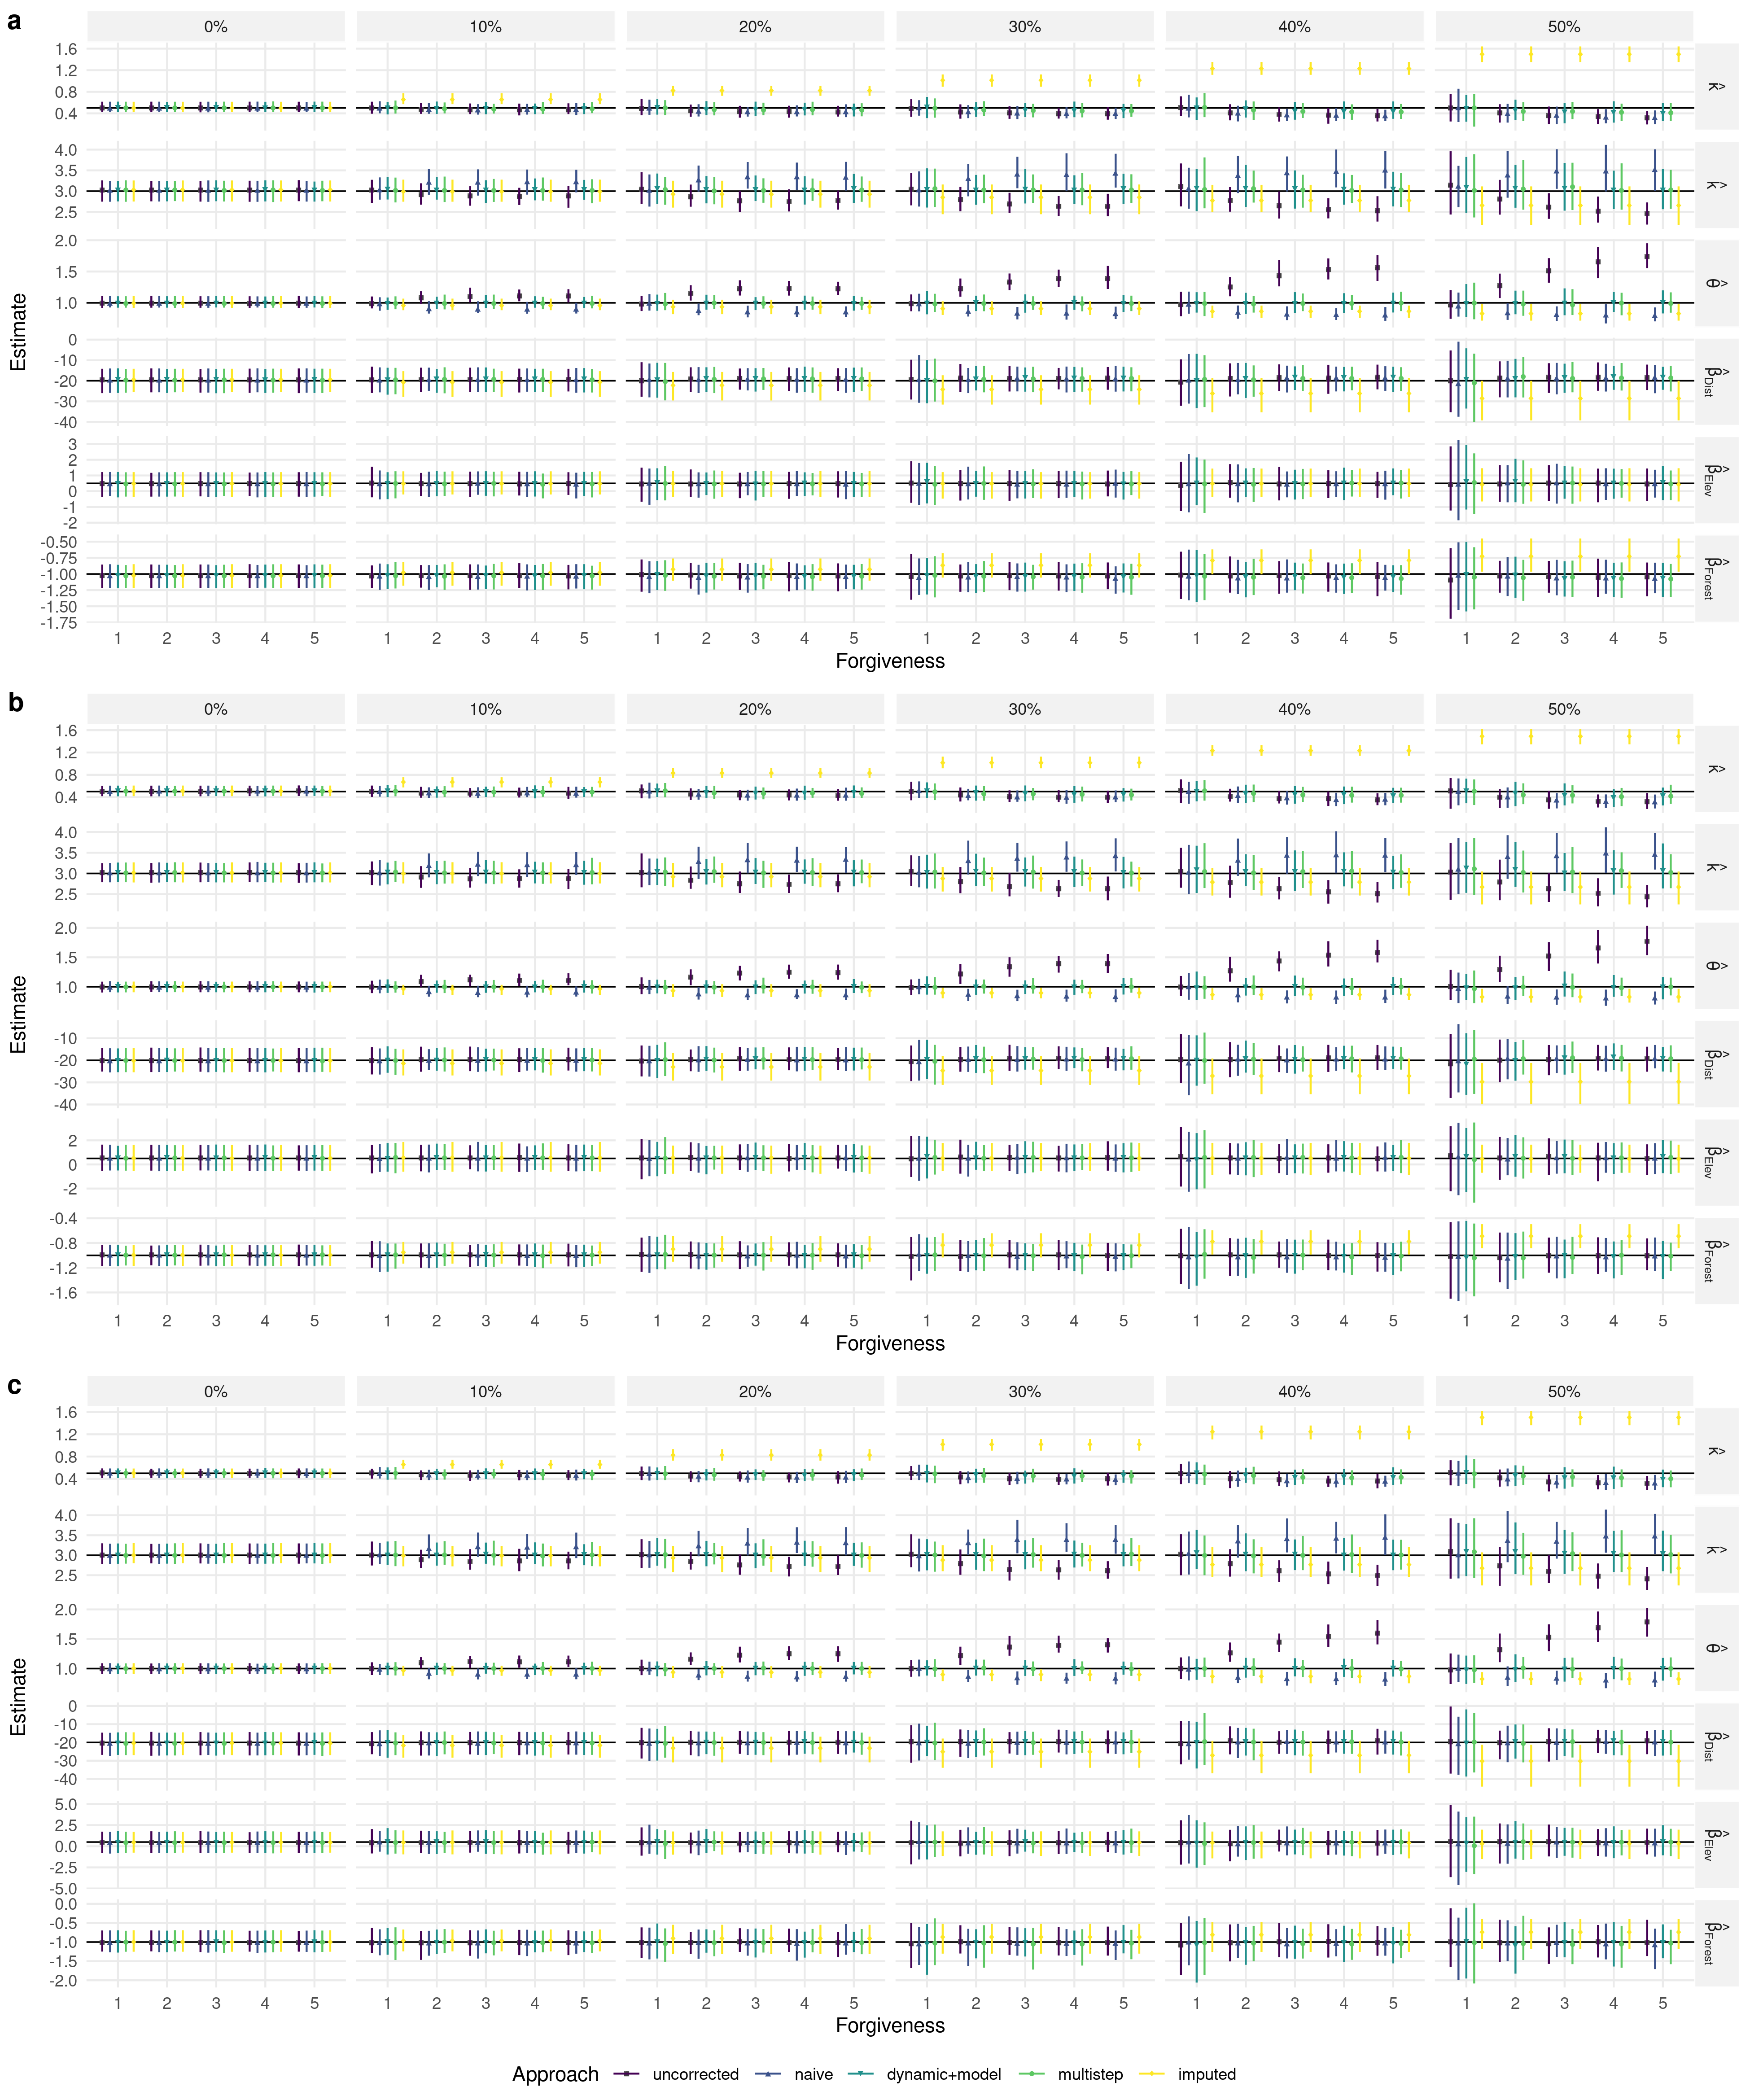
\includegraphics[width = 0.9\textwidth]{Figures/ModelComparisonAppendix.png}
  \caption{Parameter estimates across different autocorrelation scenarios (5,
  10, 20; panels a, b, and c) and missingness levels (0\% - 50\%; from left
  to right). True simulation parameters are indicated by the solid black
  lines. Parameter estimates from the different approaches are given by the
  colored symbols, and their bootstrap 95\% CIs across 100 replicates
  by the colored lines.}
  \label{ModelComparison}
  \end{center}
\end{figure}

%------------------------------------------------------------------------------
%	Appendix S5:
%------------------------------------------------------------------------------
\newpage
\section{Case Study Covariates}

\begin{figure}[!ht]
  \begin{center}
  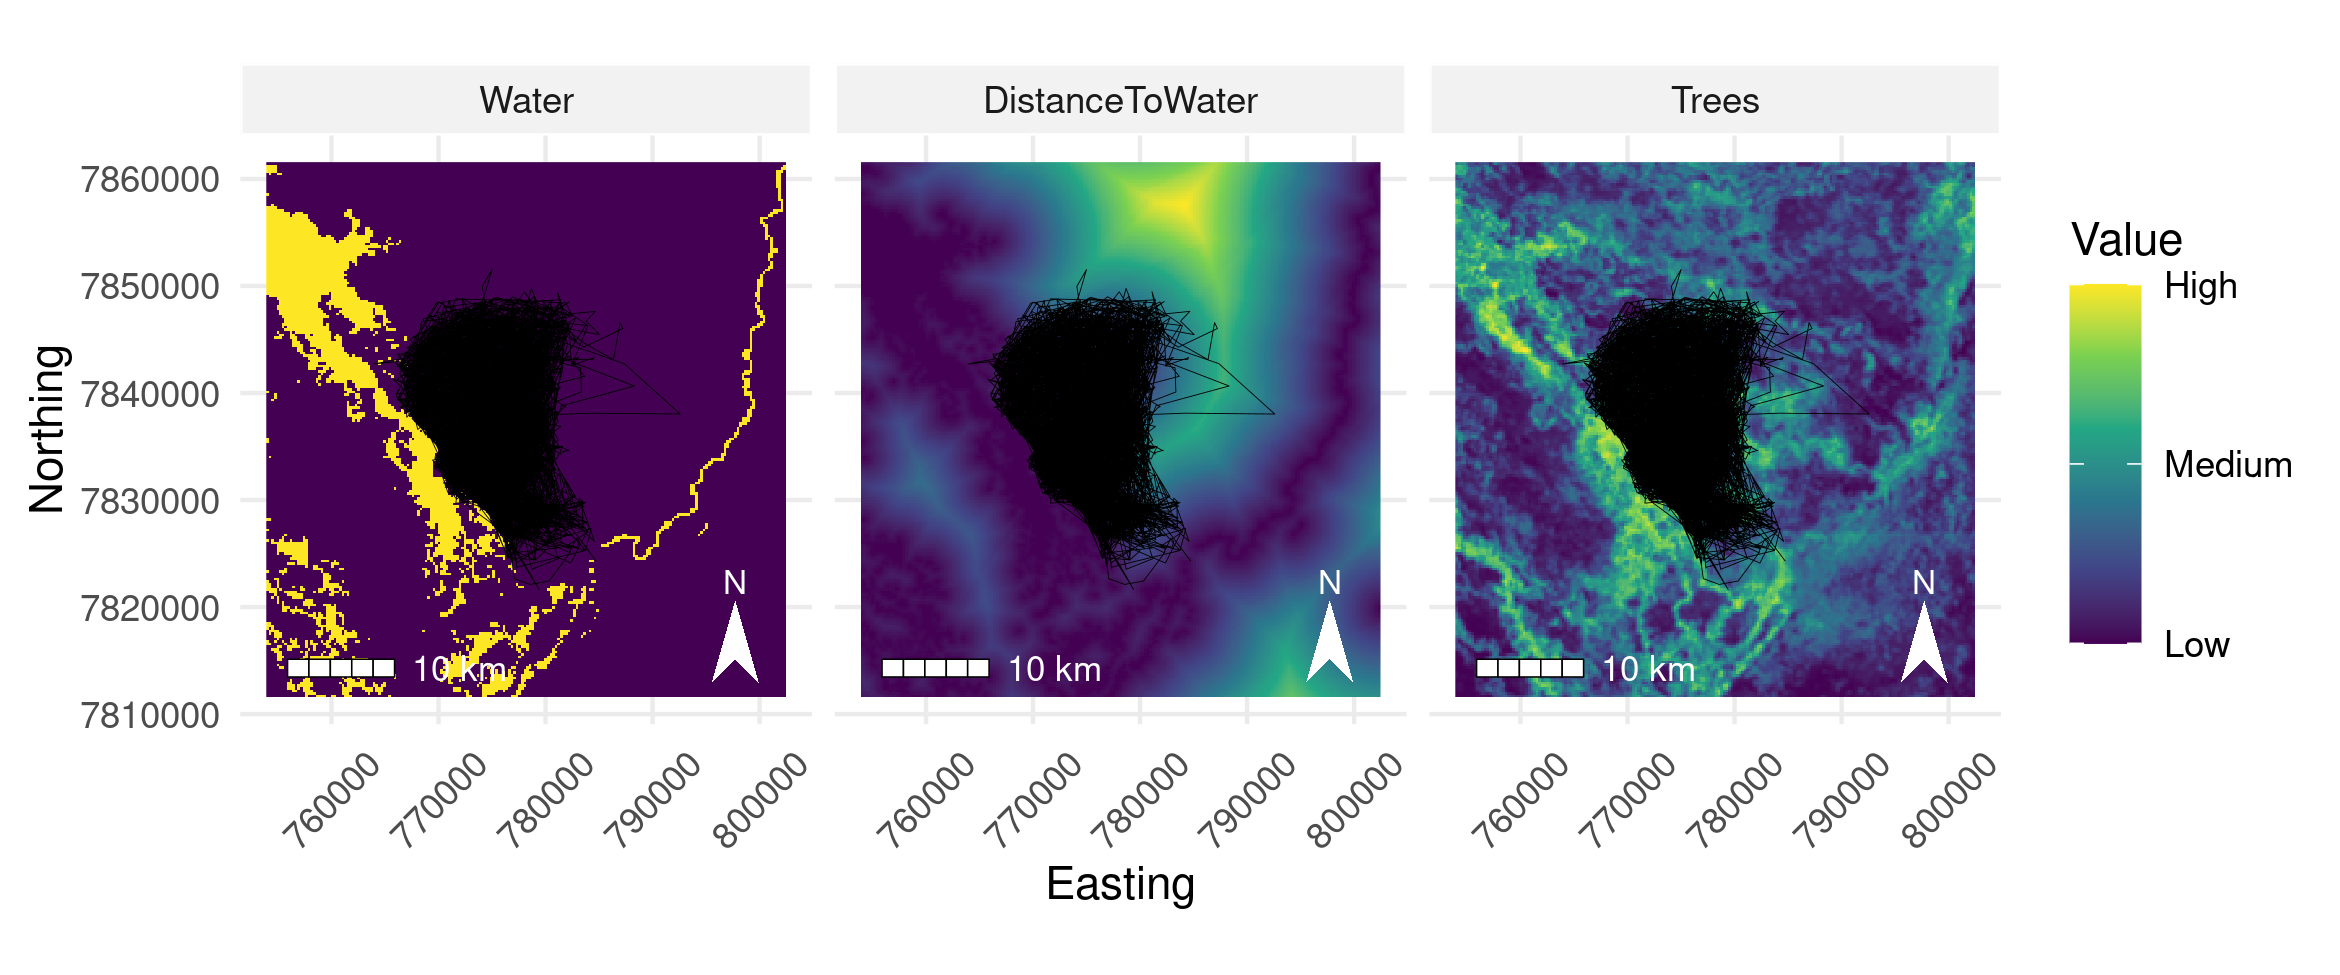
\includegraphics[width = \textwidth]{Figures/CaseStudyCovariates.png}
  \caption{Covariates used for the case study, overlaid with the GPS data of a
  spotted hyena called ``Apollo'' (lines in black). Apollo was originally
  collared in 2007 in northern Botswana and monitored until 2011. The depicted
  area is part of the Okavango Delta, which is a massive wetland area. Data was
  projected to a local projection (EPSG:32734).}
  \label{CaseStudyCovariates}
  \end{center}
\end{figure}

%------------------------------------------------------------------------------
%	Appendix S6:
%------------------------------------------------------------------------------
\newpage
\section{Case Study Model Output}

\begin{table}[!ht]
  \begin{center}
  \caption{Model results from the case study using GPS data collected on Apollo.
  In F1, forgiveness was set to one (only 2-hour steps were considered), whereas
  in F3-S and F3-SH a forgiveness of three was employed (allowing for step
  durations of up to 6 hours). In model F3-S, the step duration was interacted
  with step descriptors. In model F3-SH, step duration was interacted with step
  descriptors and habitat covariates.}
  \label{CaseStudyTable}
    \begin{adjustbox}{max width=0.65\textwidth}
    \begin{threeparttable}[h]
      
\begin{tabular}[t]{lccc}
\toprule
Coefficient & F1 & F3-S & F3-SH\\
\midrule
sl & 0.00002 & 0.00001 & 0.00001\\
\begingroup\fontsize{8}{10}\selectfont \em{}\endgroup & \begingroup\fontsize{8}{10}\selectfont \em{(0.00001)}\endgroup & \begingroup\fontsize{8}{10}\selectfont \em{(0.00001)}\endgroup & \begingroup\fontsize{8}{10}\selectfont \em{\vphantom{1} (0.00001)}\endgroup\\
log\_sl & -0.02251 & -0.01805 & -0.01846\\
\begingroup\fontsize{8}{10}\selectfont \em{}\endgroup & \begingroup\fontsize{8}{10}\selectfont \em{(0.01862)}\endgroup & \begingroup\fontsize{8}{10}\selectfont \em{(0.0157)}\endgroup & \begingroup\fontsize{8}{10}\selectfont \em{(0.0157)}\endgroup\\
cos\_ta & 0.03166 & -0.0085 & -0.009\\
\begingroup\fontsize{8}{10}\selectfont \em{}\endgroup & \begingroup\fontsize{8}{10}\selectfont \em{(0.03055)}\endgroup & \begingroup\fontsize{8}{10}\selectfont \em{(0.02557)}\endgroup & \begingroup\fontsize{8}{10}\selectfont \em{(0.02558)}\endgroup\\
Water & -1.71418*** & -1.56915*** & -1.61501***\\
\begingroup\fontsize{8}{10}\selectfont \em{}\endgroup & \begingroup\fontsize{8}{10}\selectfont \em{(0.20628)}\endgroup & \begingroup\fontsize{8}{10}\selectfont \em{(0.13995)}\endgroup & \begingroup\fontsize{8}{10}\selectfont \em{(0.17121)}\endgroup\\
DistanceToWater & -0.00005*** & -0.00005*** & -0.00005***\\
\begingroup\fontsize{8}{10}\selectfont \em{}\endgroup & \begingroup\fontsize{8}{10}\selectfont \em{(0.00001)}\endgroup & \begingroup\fontsize{8}{10}\selectfont \em{(0.00001)}\endgroup & \begingroup\fontsize{8}{10}\selectfont \em{(0.00001)}\endgroup\\
Trees & 1.51764* & -0.2178 & 0.60764\\
\begingroup\fontsize{8}{10}\selectfont \em{}\endgroup & \begingroup\fontsize{8}{10}\selectfont \em{(0.88816)}\endgroup & \begingroup\fontsize{8}{10}\selectfont \em{(0.62517)}\endgroup & \begingroup\fontsize{8}{10}\selectfont \em{(0.75259)}\endgroup\\
sl:duration4 &  & -0.00001 & -0.00001\\
\begingroup\fontsize{8}{10}\selectfont \em{}\endgroup & \begingroup\fontsize{8}{10}\selectfont \em{}\endgroup & \begingroup\fontsize{8}{10}\selectfont \em{(0.00002)}\endgroup & \begingroup\fontsize{8}{10}\selectfont \em{\vphantom{1} (0.00002)}\endgroup\\
sl:duration6 &  & -0.00004** & -0.00004**\\
\begingroup\fontsize{8}{10}\selectfont \em{}\endgroup & \begingroup\fontsize{8}{10}\selectfont \em{}\endgroup & \begingroup\fontsize{8}{10}\selectfont \em{(0.00002)}\endgroup & \begingroup\fontsize{8}{10}\selectfont \em{(0.00002)}\endgroup\\
log\_sl:duration4 &  & 0.08122 & 0.07978\\
\begingroup\fontsize{8}{10}\selectfont \em{}\endgroup & \begingroup\fontsize{8}{10}\selectfont \em{}\endgroup & \begingroup\fontsize{8}{10}\selectfont \em{(0.05075)}\endgroup & \begingroup\fontsize{8}{10}\selectfont \em{(0.0508)}\endgroup\\
log\_sl:duration6 &  & 0.02867 & 0.03058\\
\begingroup\fontsize{8}{10}\selectfont \em{}\endgroup & \begingroup\fontsize{8}{10}\selectfont \em{}\endgroup & \begingroup\fontsize{8}{10}\selectfont \em{(0.02471)}\endgroup & \begingroup\fontsize{8}{10}\selectfont \em{(0.02474)}\endgroup\\
cos\_ta:duration4 &  & -0.07526 & -0.07635\\
\begingroup\fontsize{8}{10}\selectfont \em{}\endgroup & \begingroup\fontsize{8}{10}\selectfont \em{}\endgroup & \begingroup\fontsize{8}{10}\selectfont \em{(0.05784)}\endgroup & \begingroup\fontsize{8}{10}\selectfont \em{(0.05788)}\endgroup\\
cos\_ta:duration6 &  & -0.16358*** & -0.16105***\\
\begingroup\fontsize{8}{10}\selectfont \em{}\endgroup & \begingroup\fontsize{8}{10}\selectfont \em{}\endgroup & \begingroup\fontsize{8}{10}\selectfont \em{(0.06055)}\endgroup & \begingroup\fontsize{8}{10}\selectfont \em{(0.06059)}\endgroup\\
Water:duration4 &  &  & 0.08548\\
\begingroup\fontsize{8}{10}\selectfont \em{}\endgroup & \begingroup\fontsize{8}{10}\selectfont \em{}\endgroup & \begingroup\fontsize{8}{10}\selectfont \em{}\endgroup & \begingroup\fontsize{8}{10}\selectfont \em{(0.34111)}\endgroup\\
Water:duration6 &  &  & 0.20782\\
\begingroup\fontsize{8}{10}\selectfont \em{}\endgroup & \begingroup\fontsize{8}{10}\selectfont \em{}\endgroup & \begingroup\fontsize{8}{10}\selectfont \em{}\endgroup & \begingroup\fontsize{8}{10}\selectfont \em{(0.46194)}\endgroup\\
DistanceToWater:duration4 &  &  & 0.00002\\
\begingroup\fontsize{8}{10}\selectfont \em{}\endgroup & \begingroup\fontsize{8}{10}\selectfont \em{}\endgroup & \begingroup\fontsize{8}{10}\selectfont \em{}\endgroup & \begingroup\fontsize{8}{10}\selectfont \em{(0.00002)}\endgroup\\
DistanceToWater:duration6 &  &  & -0.00001\\
\begingroup\fontsize{8}{10}\selectfont \em{}\endgroup & \begingroup\fontsize{8}{10}\selectfont \em{}\endgroup & \begingroup\fontsize{8}{10}\selectfont \em{}\endgroup & \begingroup\fontsize{8}{10}\selectfont \em{(0.00003)}\endgroup\\
Trees:duration4 &  &  & -0.04696\\
\begingroup\fontsize{8}{10}\selectfont \em{}\endgroup & \begingroup\fontsize{8}{10}\selectfont \em{}\endgroup & \begingroup\fontsize{8}{10}\selectfont \em{}\endgroup & \begingroup\fontsize{8}{10}\selectfont \em{(1.61148)}\endgroup\\
Trees:duration6 &  &  & -6.73474***\\
\begingroup\fontsize{8}{10}\selectfont \em{}\endgroup & \begingroup\fontsize{8}{10}\selectfont \em{}\endgroup & \begingroup\fontsize{8}{10}\selectfont \em{}\endgroup & \begingroup\fontsize{8}{10}\selectfont \em{(1.97442)}\endgroup\\
\midrule
Steps & 2,179 & 4,505 & 4,505\\
AIC & - & 47,565 & 47,564\\
\bottomrule
\end{tabular}

      \begin{tablenotes}
       \item \textit{Significance codes: * \(p < 0.10\) \quad ** \(p < 0.05\)
        \quad *** \(p < 0.01\)}
      \end{tablenotes}
    \end{threeparttable}
  \end{adjustbox}
  \end{center}
\end{table}

\ifSubfilesClassLoaded{%
  \newpage
  \begin{singlespacing}
  \ifthenelse{\boolean{usebiblatex}}{
    \begin{refcontext}[sorting=nyt]
    \printbibliography
    \end{refcontext}
  } {
    \bibliography{../LiteratureBibtex}%
  }
\end{singlespacing}
}{}

\end{document}
